\hypertarget{site-adaptatif}{%
\section{Site adaptatif ?}\label{site-adaptatif}}

\begin{itemize}
\tightlist
\item
  Surfer depuis : PC, mobiles, tablettes, tv, \ldots{}
\item
  UX : navigation avec un minimum de zoom, pan, scroll
\item
  S'adapter aux spécifités des appareils

  \begin{itemize}
  \tightlist
  \item
    orientation
  \item
    taille caractères
  \item
    modes d'interaction (ex: tactile, hover, \ldots)
  \item
    \ldots{}
  \end{itemize}
\item
  1 seul site à gérer : m.cool.com ni de cool.com/mobile
\item
  Le même contenu pour tous
\item
  Souvent basé sur la largeur de l'écran
\item
  CSS3
\item
  \emph{Responsive Web Design} (1),
  \href{https://alistapart.github.io/code-samples/responsive-web-design/ex/ex-site-FINAL.html}{Exemple}
\end{itemize}

\hypertarget{techniques}{%
\section{Techniques}\label{techniques}}

\begin{itemize}
\tightlist
\item
  Media queries : Taille de l'écran (ou sortie)
\item
  UNITES RELATIVES
\item
  Fonts : Dimensions en em
\item
  Fluid Grids : Disposition et taille des éléments en \%
\item
  Flexible images (and media) : Taille des médias en \%
\item
  Autres considérations

  \begin{itemize}
  \tightlist
  \item
    Adaptatif avec
    \href{https://blog.atolcd.com/adaptive-design-versus-responsive-design/}{grilles
    fixes}
  \item
    \href{https://browserdiet.com/}{Performances} : tps chargement,
    requêtes inutiles, \ldots{}
  \item
    Transitions CSS
  \item
    \ldots{}
  \end{itemize}
\item
  \href{https://webdesignerwall.com/tutorials/responsive-design-in-3-steps}{Exemple}
\end{itemize}

\hypertarget{media-queries7}{%
\section{\texorpdfstring{\href{https://developer.mozilla.org/fr/docs/CSS/Media_queries}{Media
Queries}}{Media Queries}}\label{media-queries7}}

\begin{itemize}
\tightlist
\item
  media type :
  \textenglish{\texttt{all,\ screen,\ print,\ tv,\ braille,\ handheld,\ ...}}
\end{itemize}

\begin{english}

\begin{Shaded}
\begin{Highlighting}[]
\KeywordTok{\textless{}link}\OtherTok{ rel=}\StringTok{"stylesheet"}\OtherTok{ type=}\StringTok{"text/css"}\OtherTok{ href=}\StringTok{"style.css"}\OtherTok{ media=}\StringTok{"screen"} \KeywordTok{/\textgreater{}}
\KeywordTok{\textless{}link}\OtherTok{ rel=}\StringTok{"stylesheet"}\OtherTok{ type=}\StringTok{"text/css"}\OtherTok{ href=}\StringTok{"printfriendly.css"}\OtherTok{ media=}\StringTok{"print"} \KeywordTok{/\textgreater{}}
\end{Highlighting}
\end{Shaded}

\end{english}

\begin{itemize}
\tightlist
\item
  media query

  \begin{enumerate}
  \def\labelenumi{\arabic{enumi}.}
  \tightlist
  \item
    dans élément link
  \end{enumerate}

  \begin{english}

\begin{Shaded}
\begin{Highlighting}[]
\KeywordTok{\textless{}link}\OtherTok{ rel=}\StringTok{"stylesheet"}\OtherTok{ type=}\StringTok{"text/css"}\OtherTok{ media=}\StringTok{"screen and (max{-}device{-}width: 800px)"} 
\OtherTok{href=}\StringTok{"style800.css"} \KeywordTok{/\textgreater{}}
\end{Highlighting}
\end{Shaded}

  \end{english}

  \begin{enumerate}
  \def\labelenumi{\arabic{enumi}.}
  \setcounter{enumi}{1}
  \tightlist
  \item
    dans une feuille de style
  \end{enumerate}

  \begin{english}

\begin{Shaded}
\begin{Highlighting}[]
    \PreprocessorTok{\#nav}\NormalTok{ \{}\KeywordTok{float}\NormalTok{: }\DecValTok{right}\OperatorTok{;}\NormalTok{\}}
            \PreprocessorTok{\#nav}\NormalTok{ ul \{}\KeywordTok{list{-}style}\NormalTok{: }\DecValTok{none}\OperatorTok{;}\NormalTok{\}}
        \ImportTok{@media} \DecValTok{screen} \KeywordTok{and}\NormalTok{ (}\KeywordTok{min{-}width}\NormalTok{: }\DecValTok{400}\DataTypeTok{px}\NormalTok{) }\KeywordTok{and}\NormalTok{ (}\KeywordTok{orientation}\NormalTok{: }\DecValTok{portrait}\NormalTok{)}
\NormalTok{            \{}
                    \PreprocessorTok{\#nav}\NormalTok{ li \{}\KeywordTok{float}\NormalTok{: }\DecValTok{right}\OperatorTok{;} \KeywordTok{margin}\NormalTok{: }\DecValTok{0} \DecValTok{0} \DecValTok{0} \DecValTok{.5}\DataTypeTok{em}\OperatorTok{;} \KeywordTok{border}\NormalTok{:}\DecValTok{1}\DataTypeTok{px} \DecValTok{solid} \ConstantTok{\#000000}\OperatorTok{;}\NormalTok{\}}
\NormalTok{            \}}
        \ImportTok{@media} \DecValTok{screen} \KeywordTok{and}\NormalTok{ (}\KeywordTok{min{-}width}\NormalTok{: }\DecValTok{800}\DataTypeTok{px}\NormalTok{)}
\NormalTok{            \{}
                \PreprocessorTok{\#nav}\NormalTok{ \{ }\KeywordTok{width}\NormalTok{: }\DecValTok{200}\DataTypeTok{px}\OperatorTok{;}\NormalTok{ \}}
                   \PreprocessorTok{\#nav}\NormalTok{ li \{}\KeywordTok{float}\NormalTok{: }\DecValTok{left}\OperatorTok{;} \KeywordTok{margin}\NormalTok{: }\DecValTok{0} \DecValTok{0} \DecValTok{0} \DecValTok{.5}\DataTypeTok{em}\OperatorTok{;} \KeywordTok{border}\NormalTok{: }\DecValTok{none}\OperatorTok{;}\NormalTok{\}}
\NormalTok{            \}}
\end{Highlighting}
\end{Shaded}

  \end{english}

  \begin{enumerate}
  \def\labelenumi{\arabic{enumi}.}
  \setcounter{enumi}{2}
  \tightlist
  \item
    Règle CSS import
  \end{enumerate}

  \begin{english}

\begin{Shaded}
\begin{Highlighting}[]
    \ImportTok{@import} \FunctionTok{url(}\StringTok{style600min.css}\FunctionTok{)} \DecValTok{screen} \KeywordTok{and}\NormalTok{ (}\KeywordTok{min{-}width}\NormalTok{: }\DecValTok{600}\DataTypeTok{px}\NormalTok{)}\OperatorTok{;}
\end{Highlighting}
\end{Shaded}

  \end{english}
\end{itemize}

\hypertarget{media-queries7-1}{%
\section{\texorpdfstring{\href{https://developer.mozilla.org/fr/docs/CSS/Media_queries}{Media
Queries}}{Media Queries}}\label{media-queries7-1}}

\begin{english}

\begin{Shaded}
\begin{Highlighting}[]
\NormalTok{    width, height, device{-}width, device{-}height, orientation, aspect{-}ratio, }
\NormalTok{    device{-}aspect{-}ratio, color, color{-}index, monochrome, resolution, scan, grid}
\end{Highlighting}
\end{Shaded}

\end{english}

\begin{itemize}
\tightlist
\item
  Règles CSS selon medium (souvent min-, max-width)
\item
  Opérateurs : only, not, and
\item
  Au moins 3 layouts : mobile, tablet, desktop
\item
  Resolution breakpoints : 320, 480, 600, 768, 1024, 1200px
\item
  Souvent ces règles sont utilisées pour :

  \begin{itemize}
  \tightlist
  \item
    agrandir la taille du texte
  \item
    agrandir la taille des zones cliquables (utilisation au doigt)
  \item
    faire passer le contenu sur une seule colonne
  \item
    masquer ou afficher des éléments spécifiques
  \item
    ajuster les dimensions et marges
  \end{itemize}
\item
  Attention à l'ordre de chargement
\end{itemize}

\hypertarget{meta-tag-viewport8}{%
\section{\texorpdfstring{Meta Tag
\href{http://blog.javierusobiaga.com/stop-using-the-viewport-tag-until-you-know-ho}{viewport}}{Meta Tag viewport}}\label{meta-tag-viewport8}}

\begin{itemize}
\tightlist
\item
  Introduit pour
  \href{https://developer.apple.com/library/content/documentation/AppleApplications/Reference/SafariWebContent/UsingtheViewport/UsingtheViewport.html}{iPhone},
  puis standard de fait

  \begin{itemize}
  \tightlist
  \item
    Par défaut, l'affichage est réduit (980px affichés sur écran 320px)
  \item
    Meta tag viewport permet de changer ce ratio
  \end{itemize}
\item
  viewport : display area ≠ rendering surface
\item
  Mobiles : viewport \textgreater{} écran (iphone 3 : v:980 / é:320)
\item
  Media queries comparent au viewport
\item
  Mise à jour du viewport à la taille de l'écran nécessaire :
\end{itemize}

\begin{english}

\begin{Shaded}
\begin{Highlighting}[]
\KeywordTok{\textless{}meta}\OtherTok{ name=}\StringTok{"viewport"}\OtherTok{ content=}\StringTok{"width=device{-}width; initial{-}scale=1.0"}\KeywordTok{\textgreater{}}
\end{Highlighting}
\end{Shaded}

\end{english}

\hypertarget{ruxe9sultat-cible-contexte}{%
\section{Résultat = Cible / Contexte}\label{ruxe9sultat-cible-contexte}}

\begin{figure}
\centering
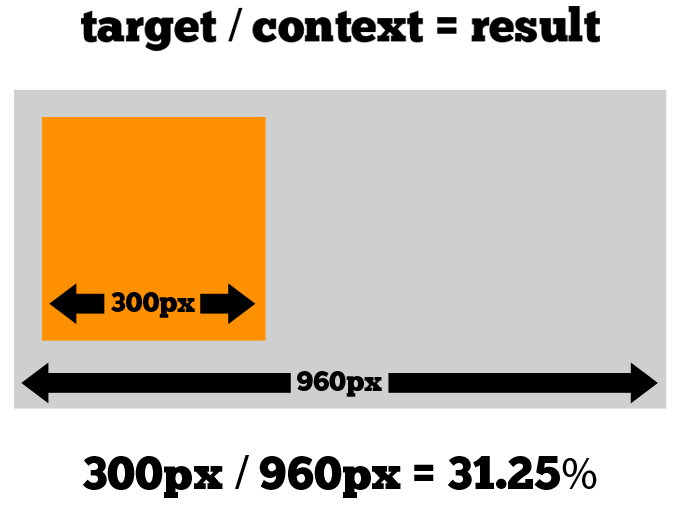
\includegraphics{src/img/target-context.png}
\caption{Target / Context}
\end{figure}

\hypertarget{texte}} dans élément html
  (16px/défaut)
\item
  \textenglish{\texttt{1em\ :\ font-size:100\%}} dans élément courant
\item
  Conversion px -\textgreater{} em :
  \textenglish{\texttt{result\ =\ target/context}}

  \begin{itemize}
  \tightlist
  \item
    ne pas arrondir
  \item
    laisser le rapport en commentaire
  \end{itemize}
\end{itemize}

\hypertarget{fluid-grids}{%
\section{Fluid Grids}\label{fluid-grids}}

\begin{itemize}
\tightlist
\item
  Layout basé sur une grille en pixel
\item
  Conversion px -\textgreater{} \% : \textbf{result = target/context}

  \begin{itemize}
  \tightlist
  \item
    ne pas arrondir
  \item
    laisser le rapport en commentaire
  \end{itemize}
\item
  Appliqué au style des divs :
\end{itemize}

\begin{english}

\begin{Shaded}
\begin{Highlighting}[]
\NormalTok{width, margin, padding, background{-}position, ...}
\end{Highlighting}
\end{Shaded}

\end{english}

\hypertarget{responsive-images}{%
\section{Responsive Images}\label{responsive-images}}

\begin{itemize}
\tightlist
\item
  Nouveautés de HTML 5

  \begin{itemize}
  \tightlist
  \item
    Eléments \textenglish{\texttt{\textless{}picture\textgreater{}}},
    \textenglish{\texttt{\textless{}source\textgreater{}}}
  \item
    Attributs \textenglish{\texttt{srcset}} et
    \textenglish{\texttt{sizes}}
  \end{itemize}
\item
  \href{http://www.smashingmagazine.com/2014/05/14/responsive-images-done-right-guide-picture-srcset/}{Besoins}

  \begin{itemize}
  \tightlist
  \item
    Écrans haute densité : \textenglish{\texttt{srcset}}
  \item
    Taille variable : \textenglish{\texttt{srcset}} et
    \textenglish{\texttt{sizes}}
  \item
    \href{http://ericportis.com/etc/smashing-mag-picture-examples/art-direction.html}{Substitution}
    et modification layout :
    \textenglish{\texttt{\textless{}picture\textgreater{},\ \textless{}source\textgreater{}}}
  \item
    Choix formats de fichiers
    \textenglish{\texttt{\textless{}picture\textgreater{}}}
  \end{itemize}
\item
  \href{https://css-tricks.com/responsive-images-youre-just-changing-resolutions-use-srcset/}{Différences}
  entre \textenglish{\texttt{\textless{}picture\textgreater{}}} et
  \textenglish{\texttt{srcset}}
\item
  \href{http://www.hteumeuleu.fr/attribut-srcset-images-responsive/}{Exemple}
  en français
\end{itemize}

\hypertarget{flexible-images}{%
\section{Flexible images}\label{flexible-images}}

\begin{itemize}
\tightlist
\item
  Eviter qu'une image ne déborde de son conteneur

  \begin{itemize}
  \tightlist
  \item
    La réduire
  \end{itemize}

  \begin{english}

\begin{Shaded}
\begin{Highlighting}[]
\NormalTok{img, embed, object, video\{ max{-}width: 100\%; \}}
\end{Highlighting}
\end{Shaded}

  \end{english}

  \begin{itemize}
  \tightlist
  \item
    La découper
  \end{itemize}

  \begin{english}

\begin{Shaded}
\begin{Highlighting}[]
\NormalTok{  .feature \{ overflow: hidden; \}}
\NormalTok{  .feature img \{ display: block; max{-}width: auto; \}}
\end{Highlighting}
\end{Shaded}

  \end{english}
\item
  Pas de standard pour servir différentes tailles de fichier
\item
  Quelques idées recensées par \emph{Smashing Magazine} (2)
\end{itemize}

\hypertarget{outils}{%
\section{Outils}\label{outils}}

\begin{itemize}
\tightlist
\item
  Tester

  \begin{itemize}
  \tightlist
  \item
    Simulateur mobile des devtools, largeur browser
  \item
    \href{https://seesparkbox.com/foundry/media_query_bookmarklet}{bookmarklet}
    pour afficher les media queries
  \item
    mais surtout tester sur mobile
  \end{itemize}
\item
  Et Après ?
  \href{http://www.lukew.com/resources/mobile_first.asp}{MOBILE FIRST},
  \href{http://offlinefirst.org/}{OFFLINE FIRST},
  \href{https://developers.google.com/web/progressive-web-apps/}{PWA}
\item
  framework ou from scratch ?
\end{itemize}

\hypertarget{ruxe9fuxe9rences}{%
\section{Références}\label{ruxe9fuxe9rences}}

\begin{itemize}
\tightlist
\item
  Exemples

  \begin{itemize}
  \tightlist
  \item
    \href{http://responsivewebdesign.com/robot/}{Site} support du
    \href{https://abookapart.com/products/responsive-web-design}{livre}
    d'Ethan Marcotte
  \item
    \href{http://mediaqueri.es/}{mediaqueri.es}
  \item
    \href{http://thenextweb.com/dd/2013/01/13/30-new-inspiring-responsive-design-websites/}{thenextweb}
  \item
    \href{https://designshack.net/articles/css/20-amazing-examples-of-using-media-queries-for-responsive-web-design/}{designshack}
  \end{itemize}
\item
  Plus loin\ldots{}

  \begin{itemize}
  \tightlist
  \item
    \href{http://johnpolacek.github.io/scrolldeck.js/decks/responsive/}{Généralités}
  \item
    \href{http://www.quirksmode.org/blog/archives/2010/09/combining_meta.html}{viewport
    et media queries}
  \item
    D'autres techniques, liste de Smashing magazine (2)
  \item
    Améliorer la
    \href{http://csswizardry.com/2013/01/front-end-performance-for-web-designers-and-front-end-developers/}{performance}
  \item
    \href{https://24ways.org/2014/making-sites-more-responsive-responsibly/}{Making
    sites more responsive, responsibly}

    \begin{itemize}
    \tightlist
    \item
      Workshop
      \href{https://www.slideshare.net/caillou/2013-03-webtuesday-responsive}{Pierre
      Spring} 26.02.13
    \end{itemize}
  \end{itemize}
\end{itemize}

\hypertarget{pratique}{%
\section{Pratique}\label{pratique}}

\begin{itemize}
\tightlist
\item
  Tester les exemples sur un mobile
\item
  Comprendre les sources
\item
  Présentation adaptative de votre équipe de projet
\end{itemize}

\hypertarget{sources}{%
\section*{Sources}\label{sources}}
\addcontentsline{toc}{section}{Sources}

\hypertarget{refs}{}
\begin{cslreferences}
\leavevmode\hypertarget{ref-alistapart:rwd}{}%
1. MARCOTTE, Ethan. Responsive Web Design. {[}en~ligne{]}. 25 mai 2010.
{[}Consulté~le~6~novembre~2017{]}. Disponible à l'adresse~:
\url{https://alistapart.com/article/responsive-web-design}

\leavevmode\hypertarget{ref-smashing:rwd}{}%
2. THE SMASHING EDITORIAL. Responsive Web Design Techniques, Tools and
Design Strategies. {[}en~ligne{]}. 22 juillet 2011.
{[}Consulté~le~6~novembre~2017{]}. Disponible à l'adresse~:
\url{https://www.smashingmagazine.com/2011/07/responsive-web-design-techniques-tools-and-design-strategies/}
\end{cslreferences}
